\subsection{Model Fit}
\label{subsec:fit_results}

This section compares simulated data from our model with empirical data from Germany. We
look at observed infections (overall as well as by age group and federal state), the
spread of the B.1.1.7 mutation, vaccinations\comment[id=K]{We fit vaccinations in the
population by construction. Maybe this should go to a different section?} and rapid test
demand.

% summary of the fit
Overall, our model achieves an excellent fit of the two waves of infections with few free
parameters (Figure~\ref{fig:aggregated_fit2}. As a result the effective replication
number is similar to that reported by the RKI (see Figure~\ref{fig:fit_r_effective}).
This excellent fit is also achieved for most age groups in Germany. The fit is also good
for many German federal states. Despite, the fact that the number of performed rapid
tests and their distribution in the population result endogenously inside our model we
fit the share of the population with at least a weekly rapid test very well and err on
the side of too few individuals that have ever done a rapid test.

% observed infections
Our fit of the infection rates in Germany between October 2020 and June 2021 is
excellent. The incidence in our model matches both the levels and the shape of the
reported incidence almost perfectly. When the prevalence of the virus is high and during
phases of exponential growth, the effect of random events on the incidence is large. That
is why it's important that we rely on 30 simulation runs with different seed sequences to
average over these random differences and have a stable mean.

\begin{figure}[ht]   % observed infections with single runs
  \centering
  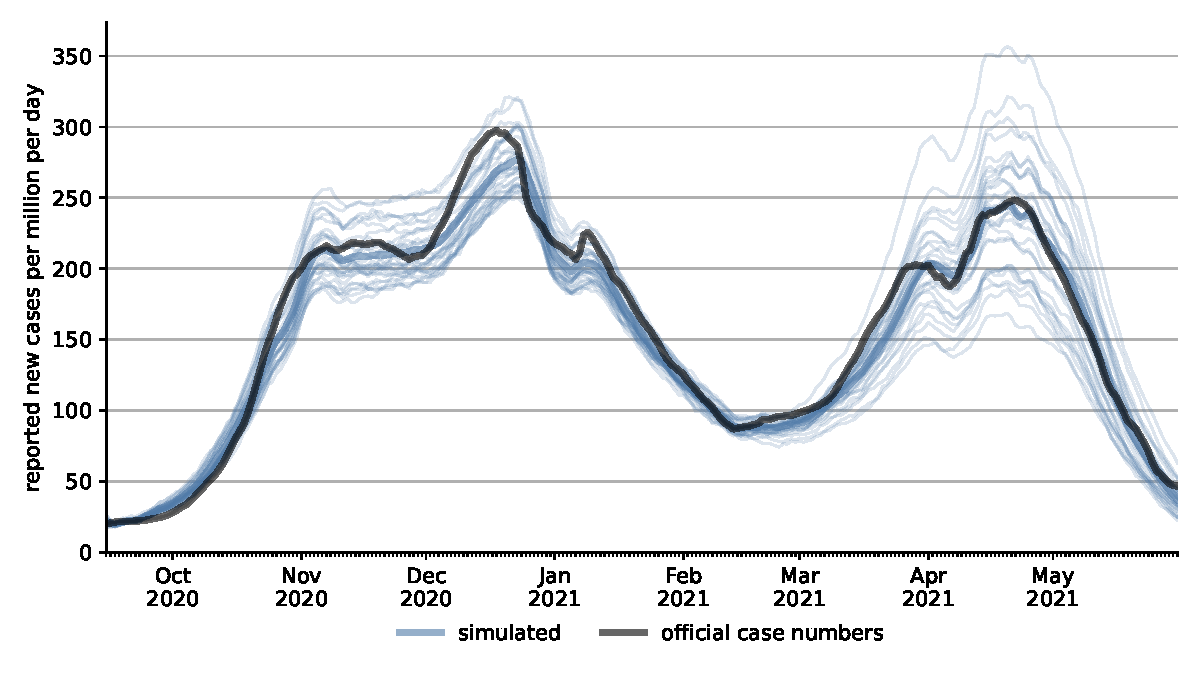
\includegraphics[width=\textwidth]{figures/results/figures/scenario_comparisons/combined_fit/full_new_known_case_with_single_runs}
  \caption{Fit Over the Full Simulation Time Frame with Single Simulation Runs}
  \floatfoot{\noindent \textit{Note:} The figure shows the daily incidence rate per
  million for the reported simulated infections rates. The mean infection rate is the
  thick blue line. Single simulation runs are plotted in lighter and thinner lines. The
  official case numbers as reported by the RKI are plotted in black. The fit is overall
  very good. The higher the mean incidence and the stronger the growth the more variance
  there is between simulation runs. We averaged over 30 simulation runs.}
  \label{fig:aggregated_fit2}
\end{figure}

% observed infections by age group
Zooming into the different age groups in Figure~\ref{fig:age_group_fit}, we can see that
our model is also able to reproduce the infection rates on this level. Differences
between the age groups allow us to identify the infection probabilities because different
age groups have contacts of different types (e.g. Mostly children go to school, the share
of workers is highest in the 35 to 59 age bracket etc.). There are very few points where
our simulated incidences and the empirical incidences do not
coincide:\comment[id=K]{@Janos: I think you can probably present this better...} Firstly,
the age group of 80 to 100 year olds due to the absence of nursing homes in our synthetic
population. Secondly, the increase in adolescents in April. We model the introduction of
rapid tests for students and do see an increase both in the observed infections and the
share of detected cases among students (see
Figure~\ref{fig:share_known_cases_by_age_group}). However, we follow \cite{Betsch2021}
that 82\% of all rapid tests are followed up with a PCR test. It is likely that that
share is higher for rapid tests that were done in schools. The last age group where our
fit does not fit the empirical curve very well is the group of 15 to 34 year olds. This
group has been touted to have a very active social life and it has often been suspected
that this age group also stayed more socially active during the pandemic. However, our
model does not include either effect because of very little data on both and hence it's
unsurprising that the actual case numbers in this group are consistently higher than our
simulated case numbers.\comment[id=K]{Does anyone have an idea why we do not match the
shape from Oct to Dec?}

\begin{figure}[ht]  % observed infections by age group
  \centering
  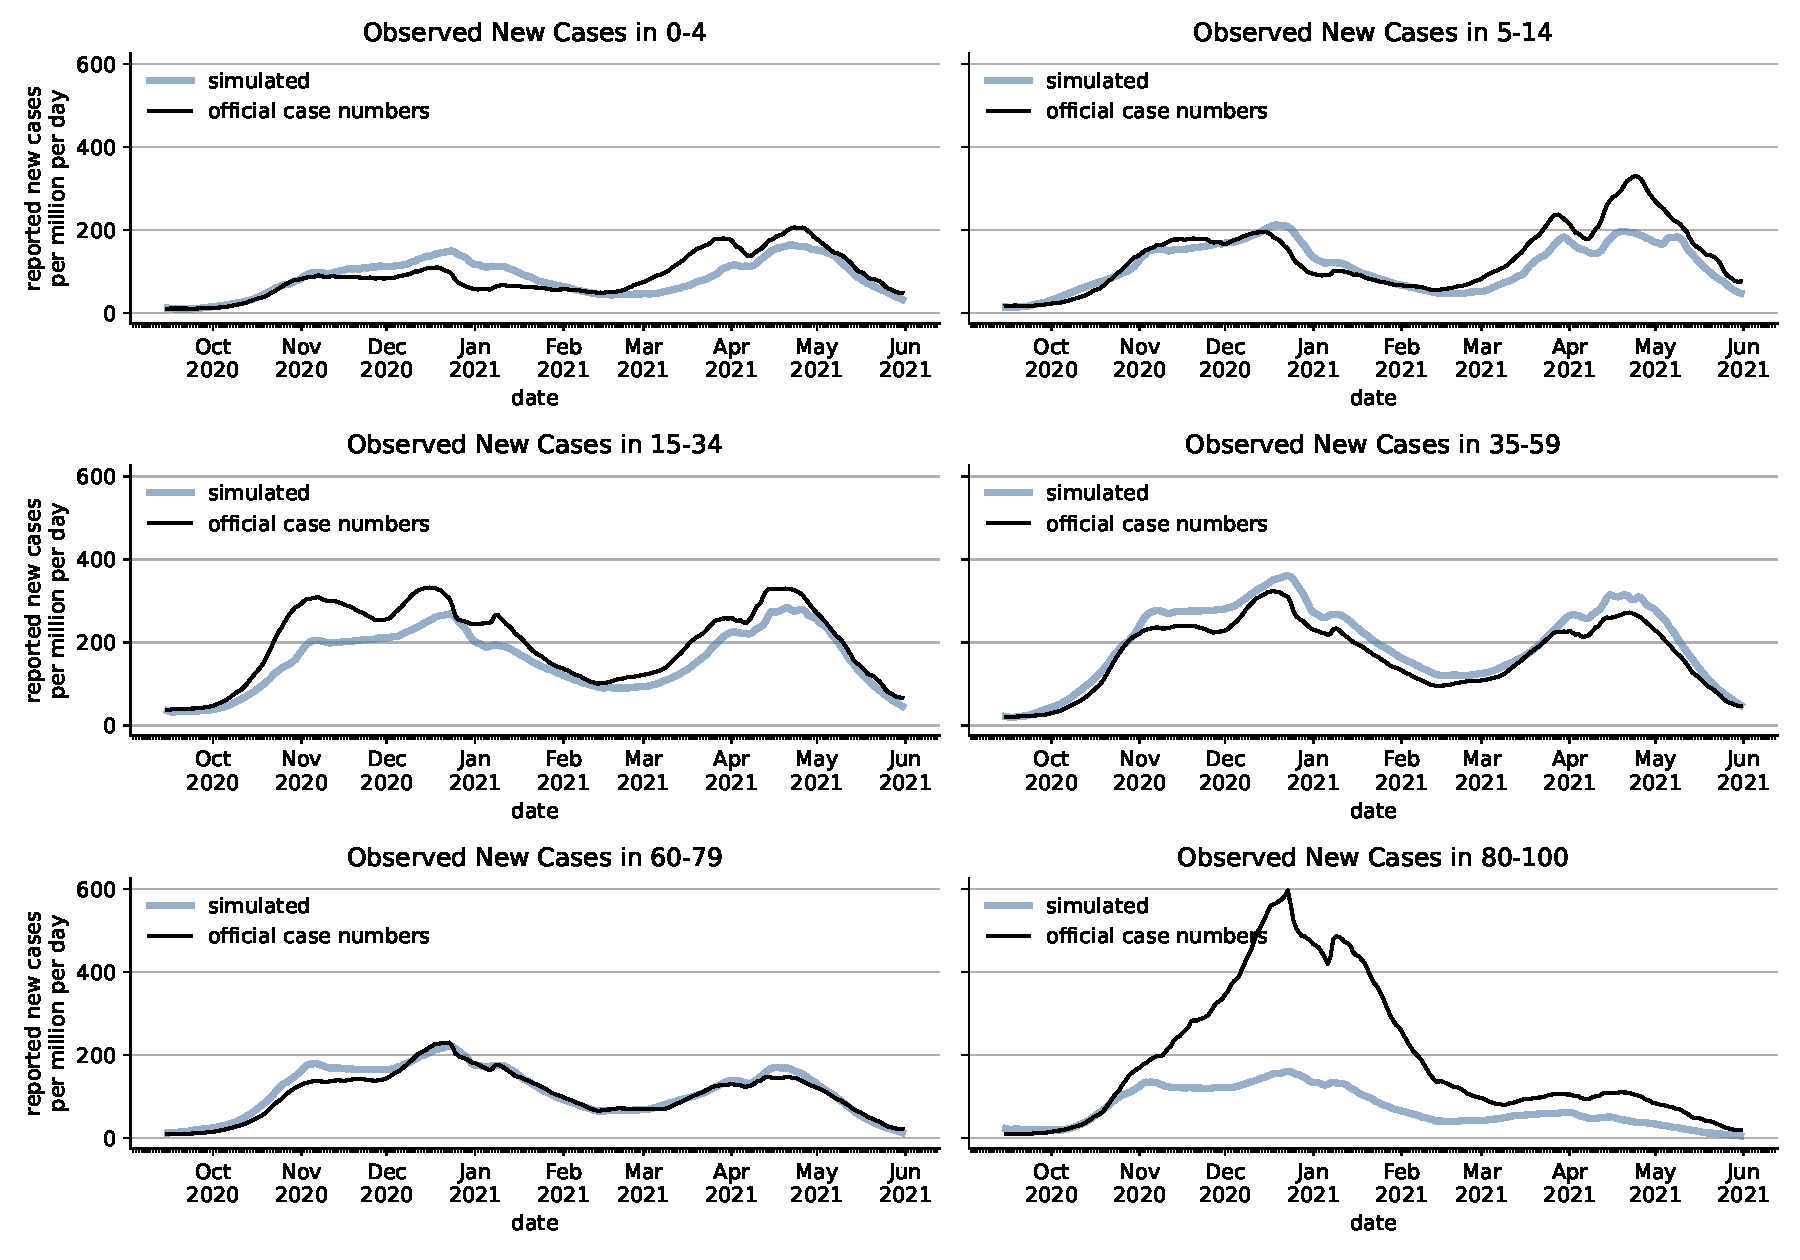
\includegraphics[width=\textwidth]{figures/results/figures/incidences_by_group/age_group_rki/full_combined_baseline_new_known_case}
  \caption{Simulated and Empirical Infections by Age Group}
  \floatfoot{\noindent \textit{Note:} The figure shows the weekly incidence rates per
  100,000 people for the reported versus the simulated infections rates for different age
  groups. The age group of individuals above 80 needs to be interpreted with caution
  because our synthetic population only includes private households, i.e. nursing homes
  are not represented in our model. They accounted for many cases and deaths in the
  winter of 2020 and many 80 to 100 year olds live in these facilities. However, the
  official data does not contain information on whether cases were nursing home
  inhabitants or not. We averaged over 30 simulation runs.}
  \label{fig:age_group_fit}
\end{figure}


\FloatBarrier

% observed infections by federal state
Our model fit is also very good for the different German federal states. This holds not
only for the large states such as North Rhine-Westphalia or Bavaria but also for many
smaller states such as Hessen or Rhineland-Palatinate. This shows that using school
vacations dates and work mobility reductions by \cite{Google2021} at the state level
combined with county and age group specific initial conditions (see
Section~\ref{sub:initial_conditions}) and county level assortativity of contacts is
sufficient to represent many local differences.  %
The fit is especially good given that our model does not aim to have a high local
resolution. For example we abstract from population density and cross-border travel. It
is, thus, unsurprising that there are states that we do not match well, such as very
thinly populated Mecklenburg-Vorpommern and Schleswig-Holstein or Saxony with its large
border to the Czech Republic that had a much higher incidence than
Germany.\comment[id=K]{The Czech Republic had very high numbers in October (max > 800)
but they fell during Nov to 220 and then climbed again to 800 by Jan 12th so that might
be only part of the answer why Saxony had such high numbers.}


\begin{figure}[ht]   % observed infections by federal state
  \centering
  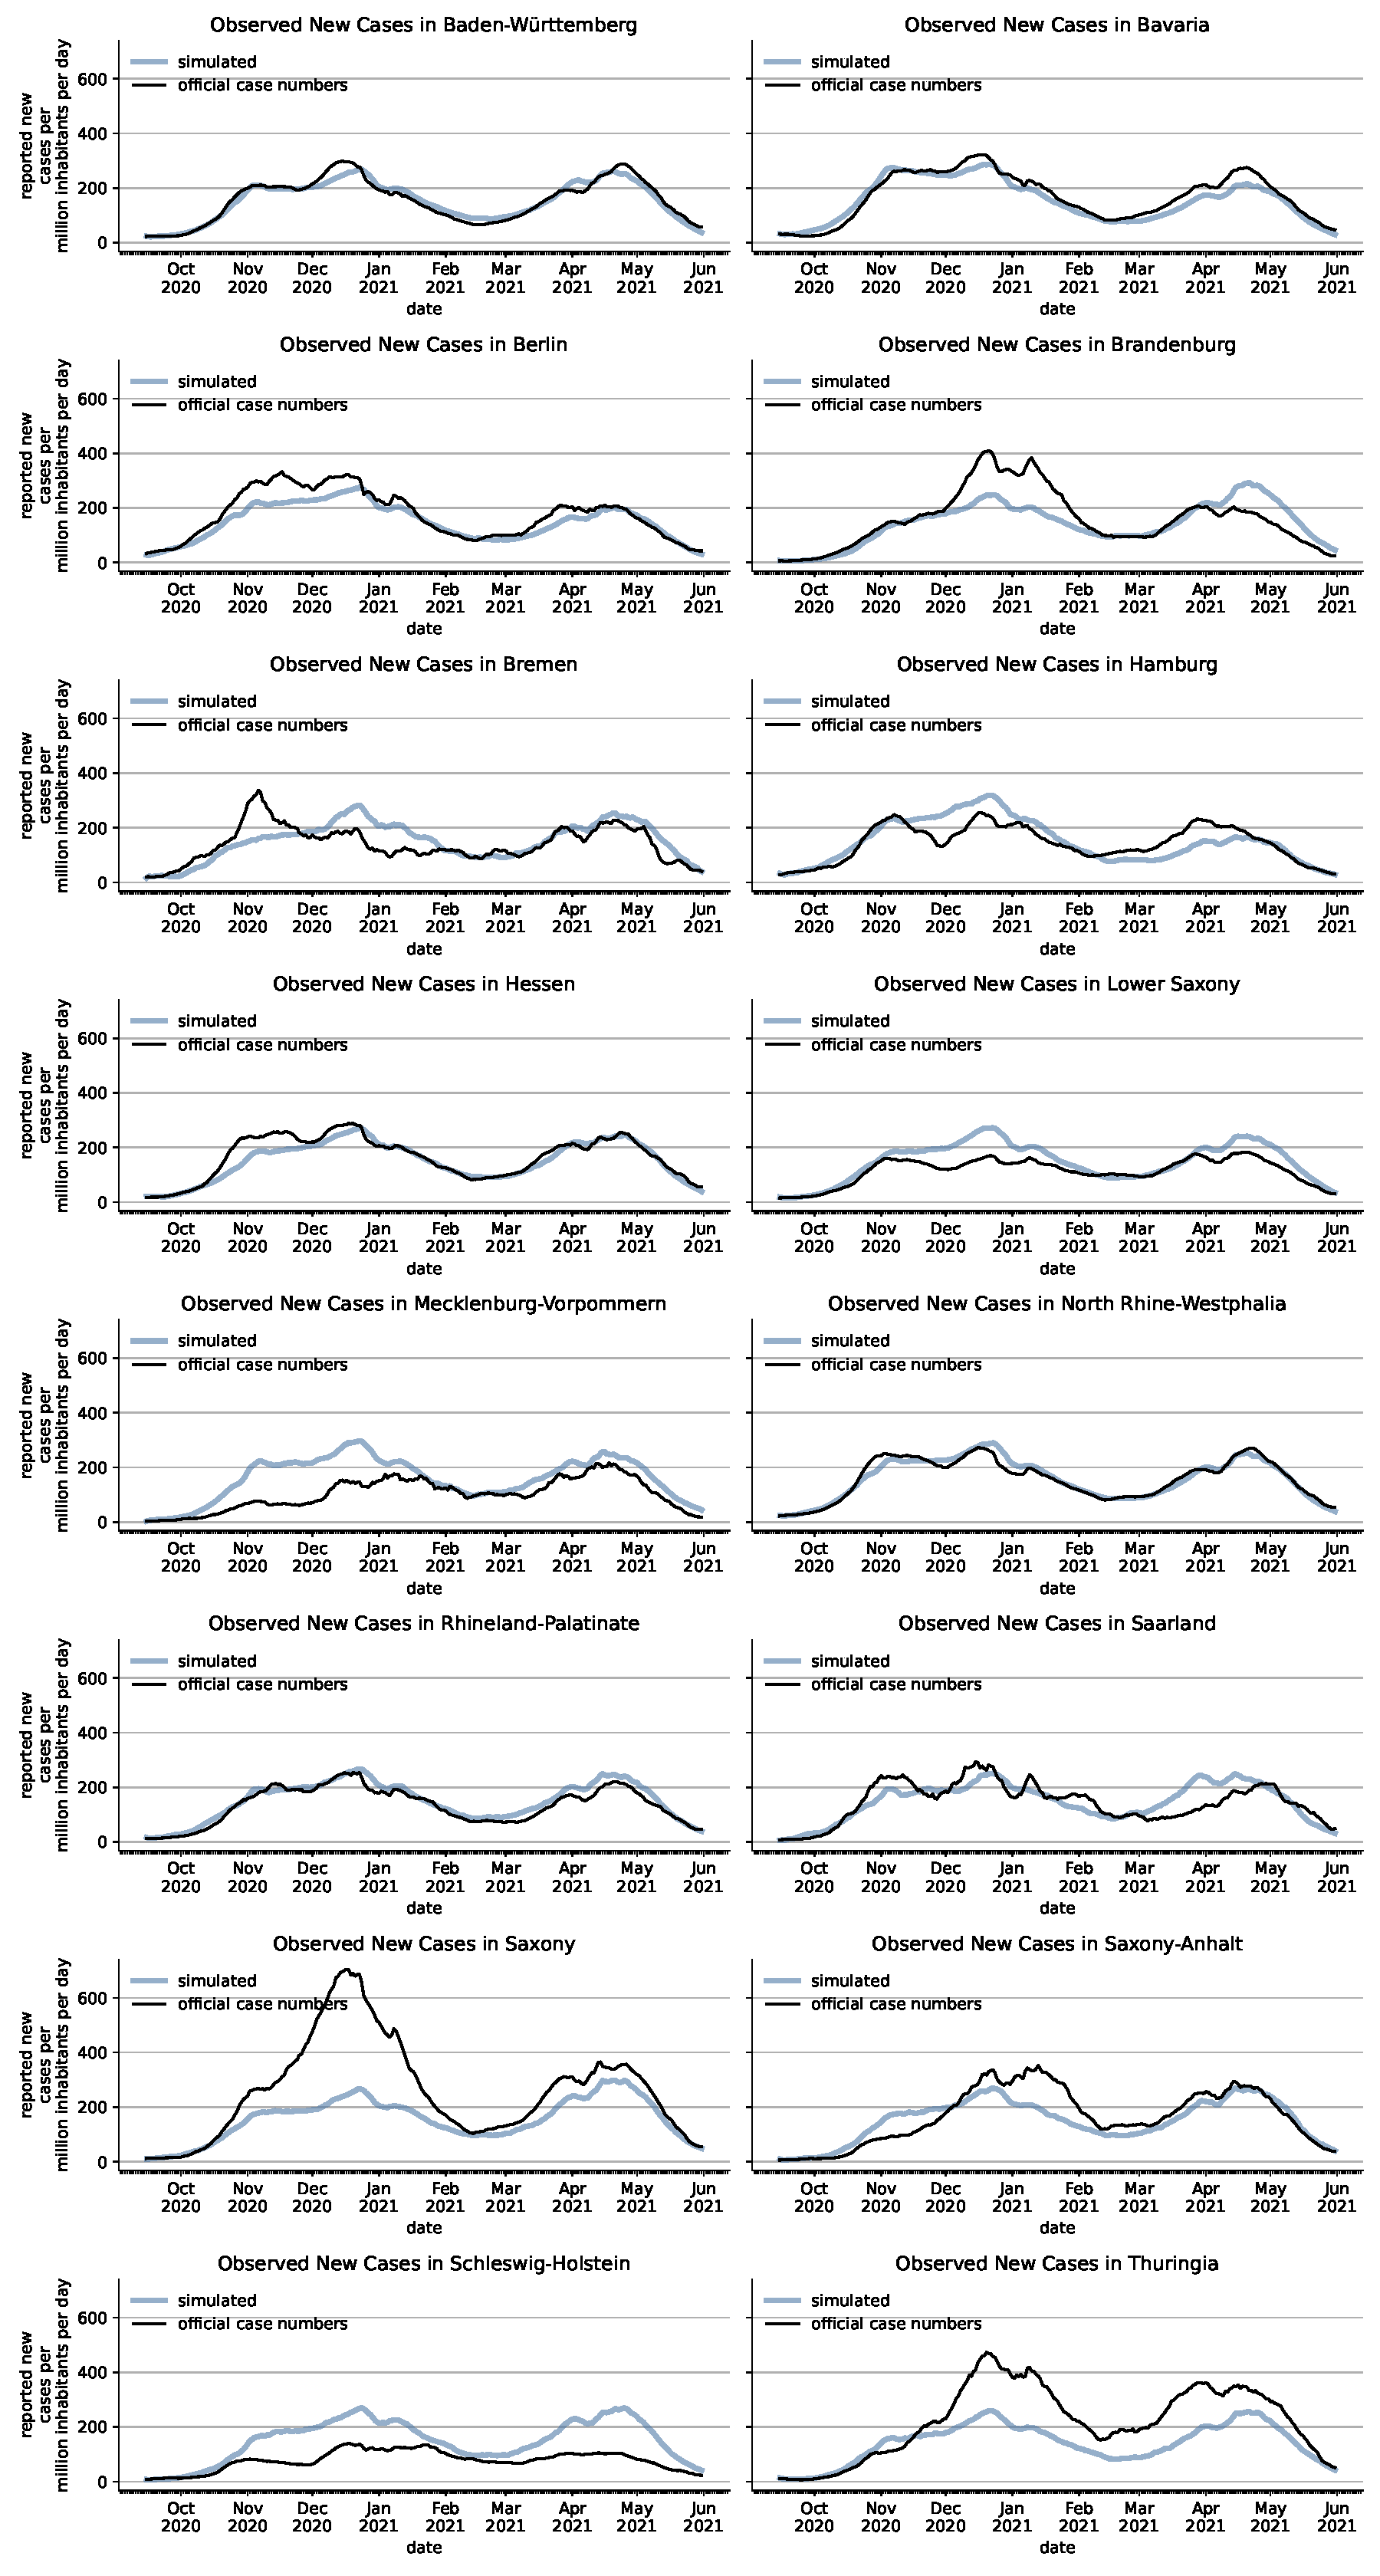
\includegraphics[height=0.95\textheight]{figures/results/figures/incidences_by_group/state/full_combined_baseline_new_known_case}
  \caption{Simulated and Empirical Infections by Federal State}
  \floatfoot{\noindent \textit{Note:} The figure shows the weekly incidence rates per
  100,000 people for the reported versus the simulated infections rates for different
  federal states. We averaged over 30 simulation runs.}
  \label{fig:state_fit}
\end{figure}

\FloatBarrier

Our fit of the effective replication number $R_t$ closely follows the values reported by
the RKI even though we calculate $R_t$ on all infected individuals not just the detected
cases. This explains why the $R_t$ in our simulations is higher during phases where the
share of detected cases falls such as in the fall of 2020 (see
Figure~\ref{fig:share_known_cases_data}) where the RKI underestimated the effective
replication number due to observing a lower share of cases and is lower than the $R_t$
reported by the RKI in spring where the share of known cases increased due to increased
rapid testing.

\begin{figure}[ht]   % R effective
  \centering
  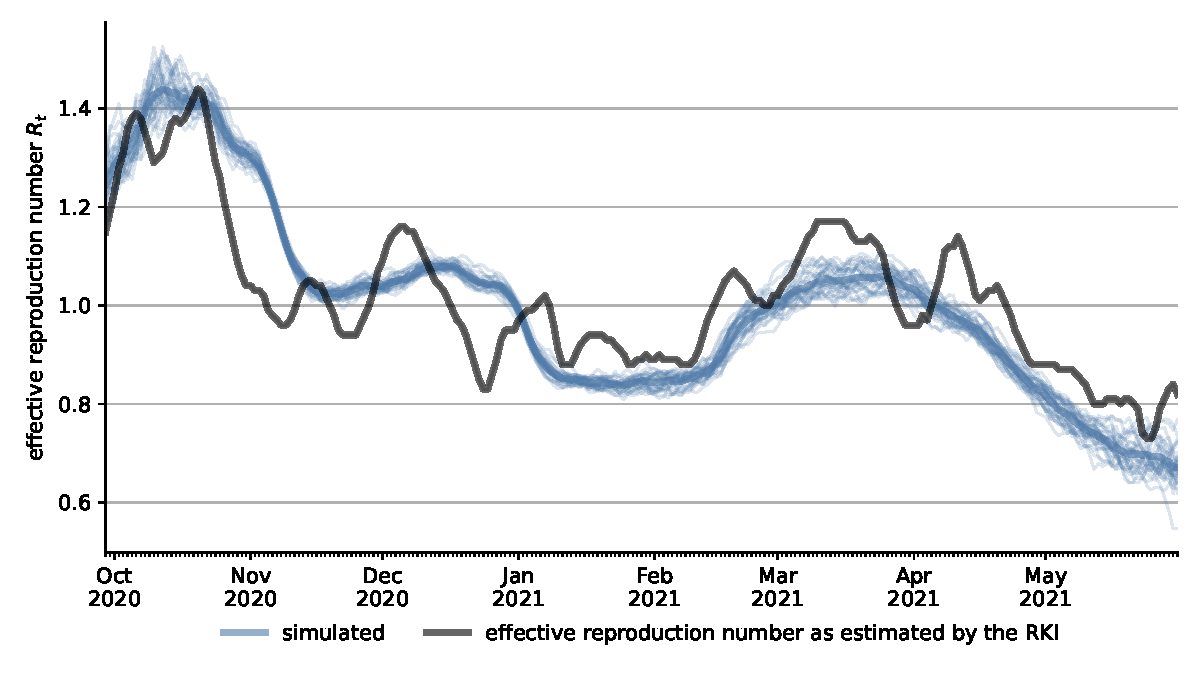
\includegraphics[width=\textwidth]{figures/results/figures/scenario_comparisons/combined_fit/full_r_effective_with_single_runs}
  \caption{Effective Replication Number $R_t$ in the Model and as Reported by the
  Robert-Koch-Institute}
  \floatfoot{\noindent \textit{Note:} The figure shows the effective replication number
  ($R_t$) as reported by the RKI and as calculated in our model. The $R_t$ gives the
  average number of new infections caused by one infected individual. The $R_t$ in our
  model broadly follows the $R_t$ reported by the RKI. Two trends stand out. Firstly, the
  RKI's $R_t$ drops faster in November. This could be due to a change in the testing
  policy that focused tests on the elderly when the second wave hit Germany and led to a
  decline in the overall share of detected cases. The second difference is from mid
  February to mid March where the RKI's reported $R_t$ increased more rapidly than that
  in our model. Here the opposite effect can be expected. During this time rapid tests
  increased strongly leading to more cases being detected. In the short term this leads
  an $R_t$ estimation that is based on detected cases to overestimate the replication
  number.}
  \label{fig:fit_r_effective}
\end{figure}

% B.1.1.7
We fit the proliferation of the B.1.1.7 variant quite exactly despite only introducing a
few cases in January as can be seen in Figure~\ref{fig:fit_share_b117}. Since we only
model B.1.1.7 and do not include other variants B.1.1.7 reaches a share of nearly 100\%
by May while the true rate plateaued at 90\% and B.1.1.7 was then replaced by B.1.617.2
as the dominant variant in June. However, B.1.1.7 still made up over 90\% of all cases in
Germany at the end of our simulation period.

\begin{figure}[ht]   % Share B.1.1.7
  \centering
  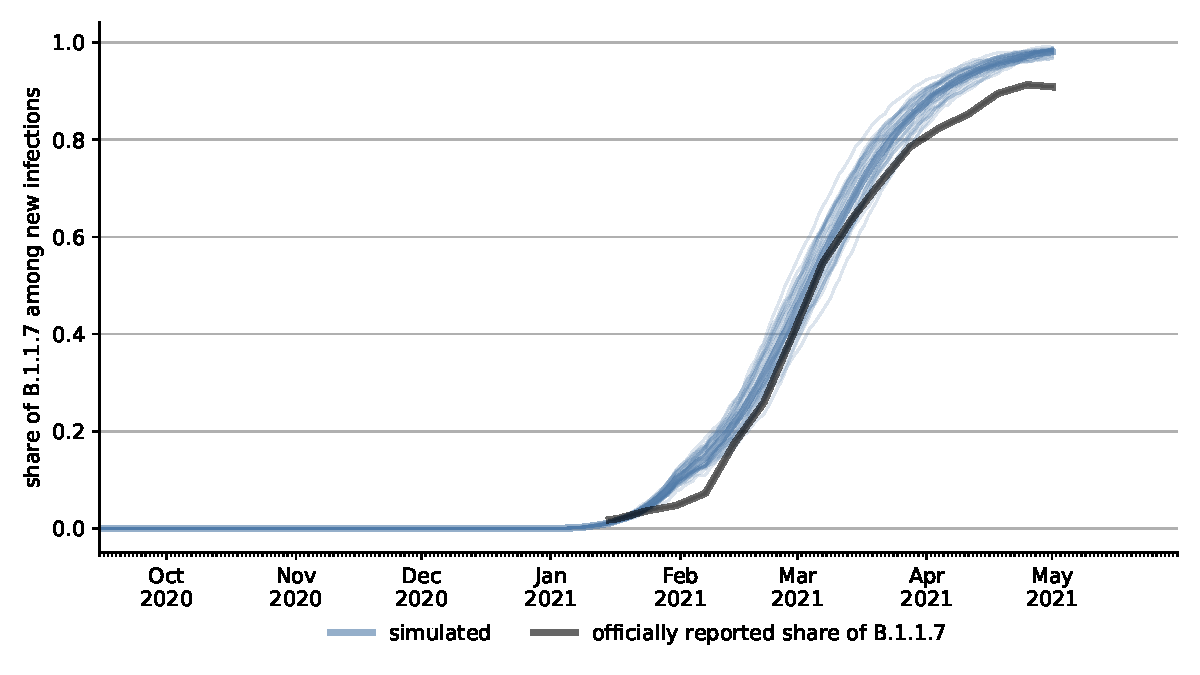
\includegraphics[width=\textwidth]{figures/results/figures/scenario_comparisons/combined_fit/full_share_b117_with_single_runs}
  \caption{Share of B.1.1.7 in the Model and as Reported by the Robert-Koch-Institute}
  \floatfoot{\noindent \textit{Note:} The figure shows the share of B.1.1.7 as
  reported by the RKI and as calculated in our model. We only introduce a few cases over
  the cause of January. From then B.1.1.7 takes over endogenously through its increased
  infectiousness. We model no other features of B.1.1.7. At most we introduce 0.75 cases per 100,000 inhabitants.}
  \label{fig:fit_share_b117}
\end{figure}

% vaccinations

The fit of the share of vaccinated individuals can be seen in
Figure~\ref{fig:fit_vaccinations}. In Germany, vaccines were rolled according to four
priority groups. The first vaccines were mostly reserved for nursing homes and some
selected professions such as first responders. Since we do not have nursing home
inhabitants in our model, we subtract the first percent of vaccinations which is
equivalent to the share of Germans living in nursing homes. Afterwards, the share of
vaccinated individuals in the population follows the German increase quite exactly. We
took great care to model the prioritization of older individuals and professions that
cannot reduce physical contact easily such as teachers or medical staff (see
Section~\ref{subsec:synthetic_population}. How the share of vaccinated individuals
develops by age group can be seen in Figure~\ref{fig:vaccinations_by_age_group}.

\begin{figure}[ht]   % fit of vaccinations
  \centering
  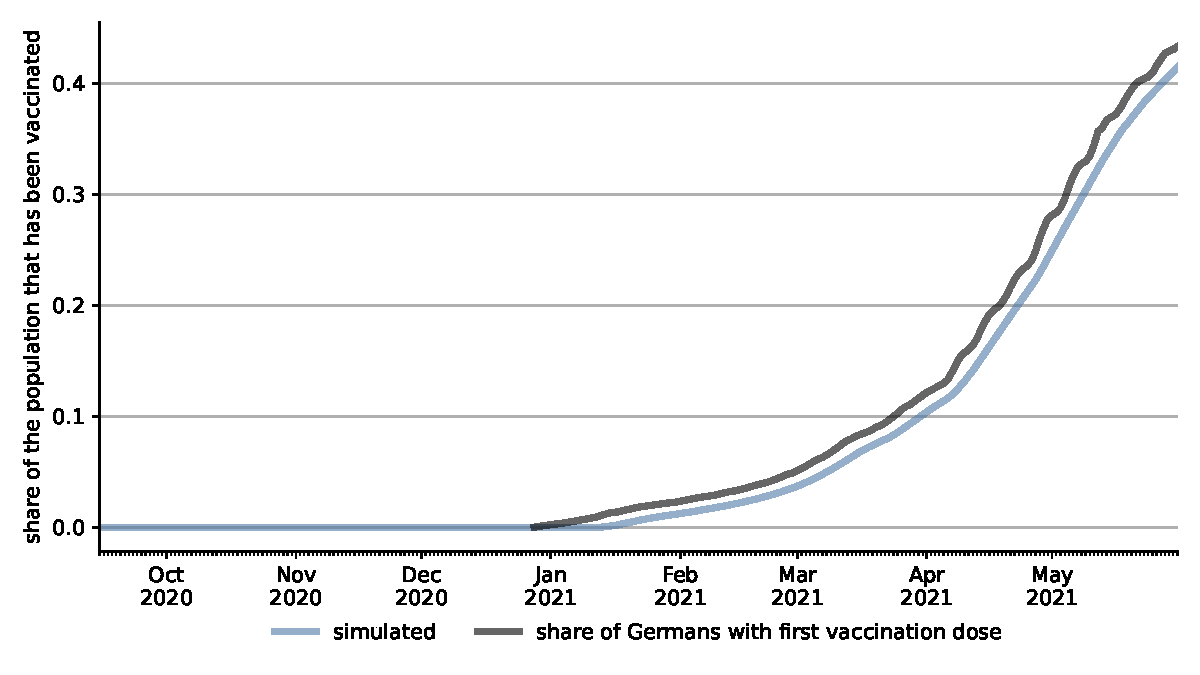
\includegraphics[width=\textwidth]{figures/results/figures/scenario_comparisons/combined_fit/full_ever_vaccinated}
  \caption{Share of Vaccinated Individuals}
  \floatfoot{\noindent \textit{Note:} The figure shows the rate of individuals that are
  vaccinated in our synthetic population versus in the general German population. Note
  that we excluded the vaccinations that were given to nursing homes, approximately the
  first percent of the German population that were vaccinated. Overall, our model covers
  a time frame that goes from zero vaccinated individuals to a state where over 40\% of
  the population are vaccinated. Our vaccinations work imperfectly but we do not model
  different vaccines nor do we distinguish between first and second shot.}
  \label{fig:fit_vaccinations}
\end{figure}

% rapid test demand
The most difficult moment to match in our model is the rapid test demand. Since we have
five different channels through which individuals demand rapid tests and many of the
demand curves are at least partially calibrated through survey data. It is therefore very
reassuring that we fit the share of individuals that do weekly rapid tests almost
perfectly. For the share of individuals that have ever done a rapid test our model is
conservative. There are two reasons for this: Firstly, we only introduce rapid tests in
2021. This is due to the small number of rapid tests in 2020 as well as a lack of data on
the number of random tests and who received them. Secondly, there is no randomness in an
individual's rapid test demand. This reduces the randomness in our model at the cost of
having less individuals that only occasionally test themselves. \comment[id=K]{Write that
this makes us underestimate the effect of random tests?} However,
Section~\ref{subsec:model_validation} shows that our results are very robust to changes
in the exact shares of individuals demanding rapid tests.

\begin{figure}[ht]     % rapid test demand
    \centering
    \caption{Share of Individuals With Rapid Tests}
    \label{fig:share_ever_rapid_test2}
    \begin{subfigure}{.55\textwidth}
        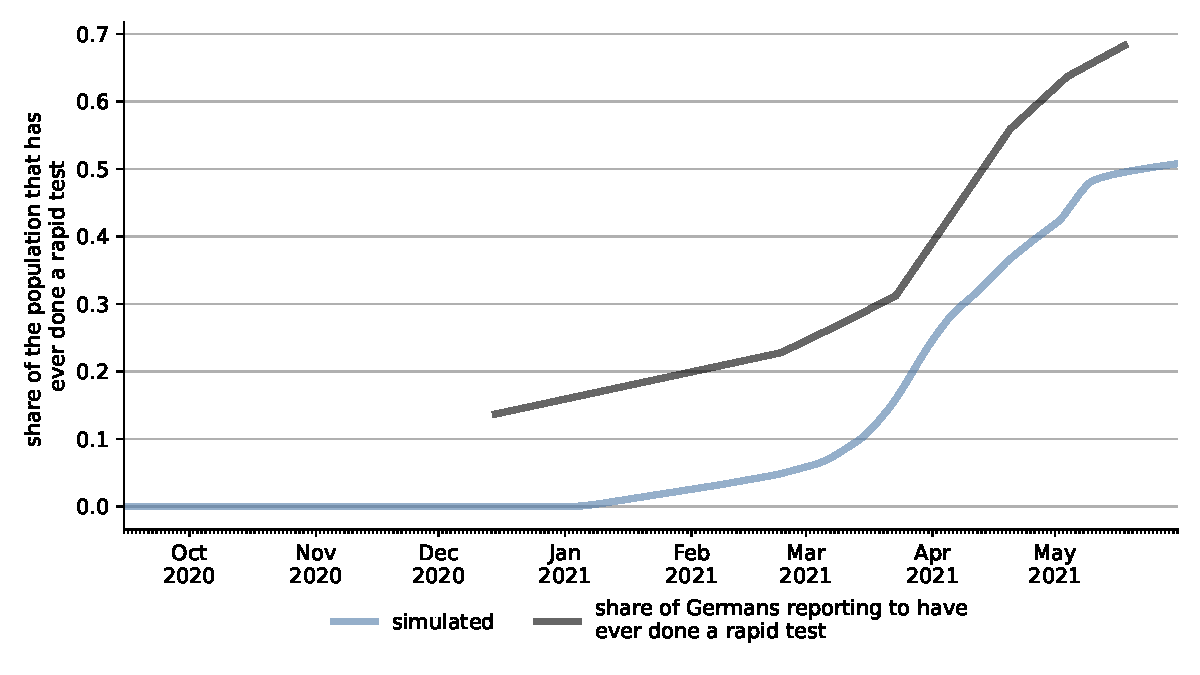
\includegraphics[width=0.9 \textwidth]{figures/results/figures/scenario_comparisons/combined_fit/full_share_ever_rapid_test}
        \caption{Share of Individuals That Have Ever Done a Rapid Test}
    \end{subfigure}%
    \begin{subfigure}{.55\textwidth}
        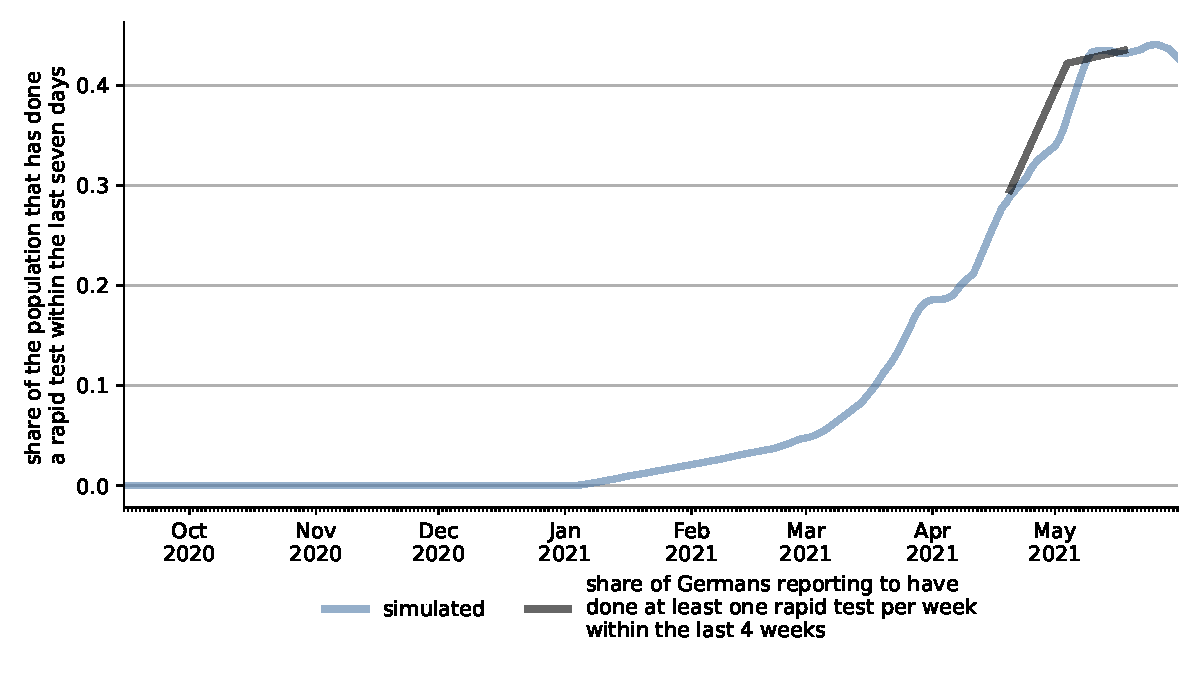
\includegraphics[width=0.9 \textwidth]{figures/results/figures/scenario_comparisons/combined_fit/full_share_rapid_test_in_last_week}
        \caption{Share of Individuals Having Done a Rapid Test in the Last Week}
    \end{subfigure}
    \label{fig:share_rapid_test_last_week2}
    \floatfoot{\noindent \textit{Note:} The figure compares the share of individuals who
        have ever done a rapid test or done a rapid test within the last week in our
        simulations to the shares reported in the
        \href{https://projekte.uni-erfurt.de/cosmo2020/web/topic/wissen-verhalten/80-schnelltests/}{COVID-19
        Snapshot Monitoring Survey}. The left panel compares the share of individuals who
        have ever done a rapid test. The right panel compares the share of individuals
        who have done a rapid test within the last seven days in our simulation compared
        to the share reporting to have done at least weekly rapid tests in the last four
        weeks in the COSMO survey. Overall our calibration of rapid tests are slightly
        conservative. The overall share is below that in the study. We fit the share of
        weekly tests quite exactly. However, the study only covers adults while our share
        also includes children who are tested very regularly when attending school.}
\end{figure}



\FloatBarrier

